\section{Discussion}

\subsection{Major findings}

    This study represents the first rigorous full structural model (i.e. explicitly incorporating various features of the CFA) for cross-linked soft tissues, and also includes a specific interaction term. An important utility of this model is its ability to separate the effects of EXLs on the fibres and matrix, so that the matrix, collagen and interaction effects could be clearly identified. This was made possible, in-part, with the use of the native–EXL matched experimental dataset and a modification to the structural model so that the uncross-linked collagen fibre responses could be mapped to the EXL configuration. As in our previous study, we found that the matrix could be well modelled as an isotropic material. However, we found that a much more linear-like response was necessary. Perhaps the most novel findings of this study were that (i) the effective collagen fibre modulus was unaffected by cross-linking and (ii) the interaction term played such a large role in stress development, often dominating the response (depending on the component and loading path being considered).
    
    
    The lack of change in the effective collagen fibre modulus has been corroborated by experimental results from Gentleman et al. \cite{gentleman_mechanical_2003}. In that study, they found a modulus range of $269.7\pm11.9$ to $ 484.7\pm76.3$ for cross-linked collagen fibres in the bovine Achilles tendon, which corresponds to the same range as another study for native collagen fibres from various sources \cite{eppell_nano_2006}. Yang et al. \cite{yang_mechanical_2008,yang_micromechanical_2007} determined that for the mechanical properties of hydrated native and cross-linked type I collagen fibrils that cross-linking the collagen fibrils with a water-soluble carbodiimide did not significantly affect the bending modulus. The work by Shen et al. \cite{shen_stress_2008} noted a modulus of $0.86\pm0.45$ GPa (range, 0.36–1.60 GPa; n = 13), in reasonable agreement with our results. Further, six of the 13 fibrils showed linear behaviour. At the tissue level, our findings are also consistent with the findings of Lee et al. \cite{lee_bovine_1989I,lee_bovine_1989II,lee_bovine_1989III}, who found no change in MTM in cross-linked pericardial tissues as in our study (table \ref{c3:tab:2}). It is interesting to note that, when using the native tissue fibre-ensemble model (equation \ref{c3:eqn:44}) on both the native and cross-linked data (figure \ref{c3:fig:5}), one can increase the fibre modulus determined from the native state to match the post-EXL data (figure \ref{c3:fig:11}a). However, this will induce a parallel increase in the MTM of approximately 75\% (figure \ref{c3:fig:11}b), which is inconsistent with the experimental findings (table \ref{c3:tab:2}). This is the case even when compensating for the effects of tissue contraction. This simple simulation lends support to the collagen modulus results (figure \ref{c3:fig:5}c).
    
    
%%%%%%%%%%%%%%%%%%%%	begin FIGURE 	%%%%%%%%%%%%%%%%%%%%
\begin{figure}
\centering
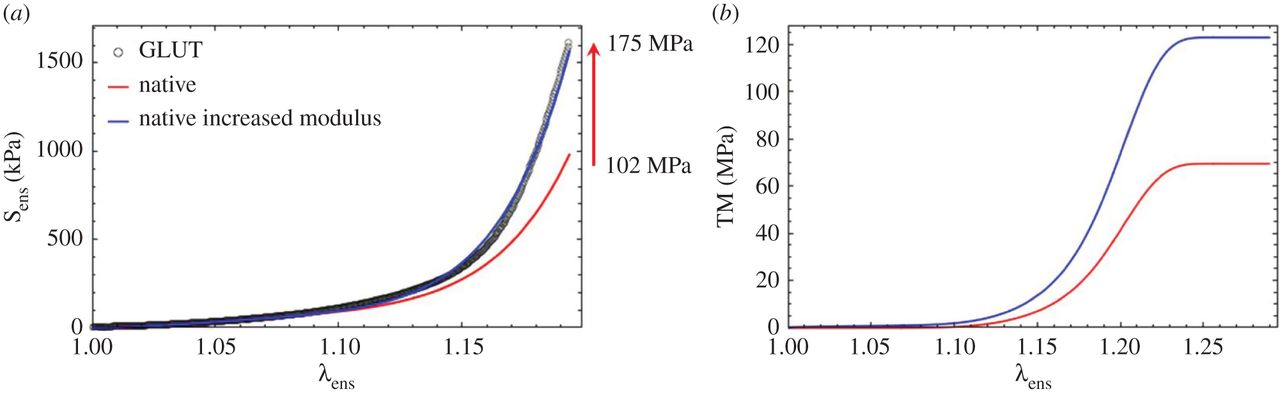
\includegraphics[width=\textwidth]{Images/chapter3/F11large.jpg}
\caption{Simulation results using the unmodified native tissue fibre-ensemble model (equation \ref{c3:eqn:44}) on both the native and cross-linked data from figure \ref{c3:fig:5}, showing that one can increase the fibre modulus determined from the native state to match the post-EXL data (a). However, this will induce a parallel increase in the MTM of approximately 75\% 
(b), which is inconsistent with the experimental findings (table \ref{c3:tab:2}). This is the case even when compensating for the effects of tissue contraction. }
\label{c3:fig:11}
\end{figure}
%%%%%%%%%%%%%%%%%%%%	 end FIGURE 	%%%%%%%%%%%%%%%%%%%%


    
    Our model results suggest that the major effect of EXL formation was not the formation of a mechanically substantial matrix or stiffening of the collagen fibres, but rather a dramatically enhanced bonding both within and between fibre ensembles. Note that our specific interaction term (equation \ref{c3:eqn:413}) captured the effects of both individual ensemble stretch and relative stretching between ensembles. This is consistent with what is known about GLUT bond formations (figure \ref{c3:fig:1}a) \cite{nimni_chemically_1987,cheung_mechanism_1985,cheung_presence_1983,cheung_mechanism_1982,cheung_mechanism_1982II}. Yet, we found that relative rotations between fibre ensembles as modelled by equation \ref{c3:eqn:415} could not capture the observed responses. The underlying structural mechanisms for this behaviour remain largely uncharacterized. One possibility is that the protein core of the proteoglycans that bind collagen fibrils become strongly cross-linked and are thus substantially stiffened, acting to more cohesively bind the collagen fibres. This is supported by findings of Liao \& Vesely \cite{liao_relationship_2004}, who observed substantial deformations of proteoglycans in mitral valve chordae under stretch. Moreover, the present model suggests that such mechanisms are strongly associated with fibre-ensemble orientation distributions. While not the final word, our results suggest that EXLs produce a stiffening effect via an isotropic matrix, with the interaction effects being the dominant effect.
    
    


\subsection{Modelling approach}

    The present approach was a direct extension of the stochastic, tissue-level meso-structural models first pioneered by Lanir \cite{lanir_constitutive_1983} and used in various applications and extensions by our group \cite{sacks_incorporation_2003,fata_insights_2014,zhang_meso_2016}. By meso-scale, we refer to the fibre-ensemble scale, which is fibre features down to approximately 100 $\mu$m. Moreover, recent evidence has demonstrated that the underlying affine kinematic assumption is valid \cite{fata_insights_2014,fan_simulation_2014}, so that the strain energy of each fibre ensemble can be kinematically connected with the macroscopic strain tensor. We took the approach to develop a more general model first, then show what components could be modified or removed entirely. Given the lack of knowledge and modelling efforts in this area, we felt this was appropriate and helped to illustrate what underlying mechanisms should be incorporated. We also considered a more extensive approach based on elastica-based theory for sinusoidal fibres based on \cite{garikipati_elastica_2008} under the assumption that EXL formation dramatically increased the fibre modulus, which ultimately proved to be unnecessary. An inter-fibre sliding model was also developed based on the relative sliding between fibres due to differences between their respective slack lengths, and used as a means to model the intra-ensemble EXL effects. However, this approach was found to be unable to capture the individual fibre-ensemble responses, suggesting that relative sliding between fibres at the ensemble level was not a major mechanism. A final question that may impact physical plausibility of the current model is convexity and physical plausibility. Lanir \cite{lanir_plausibility_1994} demonstrated that the native tissue structural model is compatible with a physically plausible response. Based on both this and the experimental observations, we focused on monotonically increasing functions of strain for all model terms to ensure physical plausibility and that convexity was maintained.
    



\subsection{Limitations and future directions}

    The current model is limited in the fact that it is quasi-static and does not account for permanent set phenomena we have observed \cite{sun_response_2004}. The homogenization method used in section \ref{c3:sec:3} is fairly standard and has been used by others and the author for some time (e.g. \cite{sacks_incorporation_2003,fata_insights_2014,fan_simulation_2014}). We have observed that for soft tissues, whose composition is dominated by a dense network of distinct fibres, especially collagen type I and elastin, these structures can be mechanically treated as fibre ensembles; that is, groups of fibres with a common orientation. The scale of the representative volume element is about 100 $\mu$m, which is sufficient to capture the salient mechanical features of the fibre ensemble. We emphasize that this is not meant to be a universal model of all types of soft tissue structures, which are very diverse for a single theoretical treatment. Rather, we focus on a sufficiently generalized approach for exogenously cross-linked dense collagenous tissues, such as pericardium, heart valves and sclera. These structures fit our approach well and also have important biomedical therapeutic applications.


    A complete understanding of the current phenomena must be based on well-characterized micro-scale events. For example, Kojic et al. \cite{kojic_numerical_1998} developed a model for fibre–fibre kinetics that uses Coulomb friction, which results in a simple and robust approach for tissue simulations. However, our knowledge of even native tissues at the micro-level remains limited. The situation remains more complicated by the fact that our knowledge of the interrelationships between the physical chemistry of EXLs and the macro-scale mechanics of collagenous tissues remains limited at the present time for more sophisticated models to be reliably attempted. To date, no material model is able to fully account for such complex observed microstructural and biological behaviour. The next steps include incorporation of the permanent set effect commonly observed in cross-linked tissues into the present model, and exploration of how alternative cross-linking methods affect macro-scale tissue behaviours.